\section{Experimental Results and Analysis}
\label{sec:result}
%-------------------------------------------------------------------------

\subsection{Best Results}

\noindent
The highest Micro-F1 score achieved so far is 93.68. This score is shown in the competition website as \cref{fig:final-score}.

\begin{figure*}
    \centering
    \begin{subfigure}{0.75\linewidth}
        %\%fbox{\rule{0pt}{2in} \rule{.9\linewidth}{0pt}}
        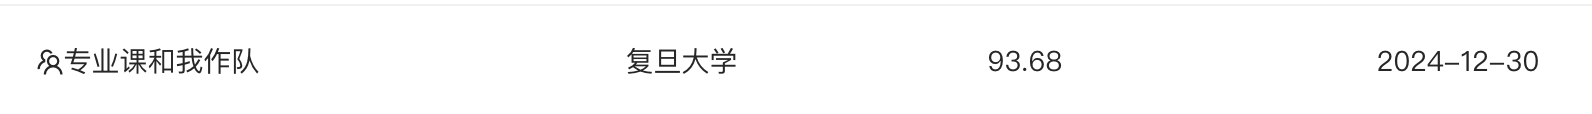
\includegraphics[width=\linewidth]{./graphs/图片14.png}
        %\caption{An example of a subfigure.}
        \label{fig:final-score1}
    \end{subfigure}
    %\hfill
    \begin{subfigure}{0.2\linewidth}
        %\fbox{\rule{0pt}{2in} \rule{.9\linewidth}{0pt}}
        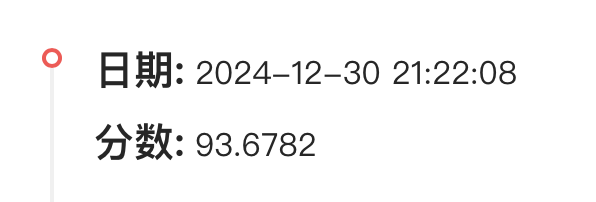
\includegraphics[width=\linewidth]{./graphs/图片15.png}
        %\caption{Another example of a subfigure.}
        \label{fig:final-score2}
    \end{subfigure}
    \caption{Screenshot of Final Score in the Competition Website}
    \label{fig:final-score}
\end{figure*}

\noindent
The experimental parameters that yielded the highest score are as follows:

\noindent
\textbf{Model:} YOLO11m

\noindent
\textbf{Number of Training Epochs:} 200

\noindent
\textbf{Unified Image Size during Training:} 800$\times$800 pixels

\noindent
\textbf{Batch:} 256

\noindent
\textbf{Prediction Confidence:} 0.2

\subsection{Result Analysis}

Based on the analysis and comparison of the performance of each model during the experiments in \cref{sec:steps}, the following conclusions can be made:

\subsubsection{Performance Analysis of Faster R-CNN}
Faster R-CNN is a precision-first two-stage object detection model that demonstrated high reliability and accuracy in this experiment, particularly in locating and classifying small targets. The experiment showed the following:

The baseline Micro-F1 score was 56.06, with limited performance when no region threshold filtering or parameter tuning was applied.

After adding region threshold filtering, the Micro-F1 score improved to 70.84, significantly enhancing the model's ability to detect small tampered regions.

However, Faster R-CNN has a slower training speed and higher computational resource demands, especially when data augmentation is used, leading to significantly increased training time. While the performance is acceptable, it is not suitable for efficient large-scale detection solutions.

\subsubsection{Performance Analysis of the YOLO Model}
YOLO models are known for their fast detection performance and strong generalization capability, particularly in small object detection and real-time applications. In the experiment:

YOLOv8n achieved a baseline Micro-F1 score of 76.84, significantly higher than Faster R-CNN.

Although YOLO11m has a larger number of parameters, it performed optimally with sufficient training (such as increasing epochs and batch size), with the Micro-F1 score exceeding 93. This indicates that YOLO models have strong adaptability to large-scale training.

\subsubsection{Horizontal Comparison Between Models}

Faster R-CNN is suitable for detection tasks that require high precision, but it has significant disadvantages in training speed and scalability.

YOLO series models, especially YOLO11m, strike a better balance between speed and accuracy, outperforming both Faster R-CNN and YOLOv8.

\subsubsection{Effectiveness of Innovative Methods}

\textbf{Region Threshold Filtering:} Introducing region threshold filtering for Faster R-CNN significantly improved the model's ability to recognize small targets, which was a key method for enhancing its performance.

\textbf{Training Parameter Adjustment:} For YOLO11m, adjusting the batch size (from 64 to 256), increasing the number of training epochs (up to 200) and increasing the $image\_size$ (up to 800) gradually improved the Micro-F1 score, indicating that larger batch training aids in enhancing model performance.

\textbf{Multi-Scale Data Augmentation:} By incorporating multi-scale data augmentation with different scaling sizes, the robustness of the model in detecting various tampering patterns was significantly improved, with the Micro-F1 score of YOLO11m rising from 90.71 to 92.25. This confirmed the importance of multi-scale multi-scale data augmentation in improving the model's generalization ability.

In summary, this experiment validated the efficiency and strong performance of YOLO11m, and the innovative methods (such as region threshold filtering and multi-scale data augmentation) significantly improved the model's Micro-F1 score, ultimately reaching 93.68. This demonstrates that through careful parameter tuning and the introduction of innovative techniques, it is possible to effectively optimize model performance and improve the accuracy of document tampering detection.

\subsection{Future Work}

Explore hybrid architectures combining the precision of Faster R-CNN and the speed of YOLO.

Experiment with larger models (\eg SAM) and evaluate their performance in more complex scenarios.

\subsection{About the Code}

A complete codebase and configuration files are provided to ensure result reproducibility.

The scripts have been optimized to accommodate various hardware environments. When using the code, the user needs to change its relative path.

The purposes of the code files in the "Codes" folder are as follows:

YOLO/eval\_yolo.py generates json file according to the YOLO model.

YOLO/transform.py turns the origin data into the right format for YOLO model.

YOLO/train.py is the YOLO training code.

YOLO/split.py divides the training data into training set and validation set randomly.

YOLO/coco.yaml is the configuration file for YOLO.

Faster R-CNN/Faster-RCNN-eval.py generates json file according to the Faster R-CNN model.

Faster R-CNN/Faster-RCNN-train.py is the Faster R-CNN training code.